\begin{lstlisting}[style=alloy]
// if there is a message in a meeting, then there is also a user with the accepted status
assert messageInMeetingEntailsAcceptedParticipation {
	all m: Meeting | #(m.chat.messages) > 0 implies (some mp: MeetingParticipation | mp.meeting = m and mp.responseStatus = Accepted)
}

// the arriving and leaving travel of a meetingParticipation are never equal
assert arrivingAndLeavingTravelAreDifferent {
	no mp: MeetingParticipation | mp.arrivingTravel = mp.leavingTravel
}

// the presence of a single non consistent meeting implies that is has been made inconstistent by the presence of a non doable break
assert singleInconsistentMeetingEntailsNotDoableBreak {
	#{mp: MeetingParticipation | mp.isMeetingConsistent = False} = 1 implies #{b: Break | b.isDoable = False} > 0
}

pred showUser {
	#User > 1
	#Break > 1
	#Status > 1
	#SocialAccount > 1
	#Group > 1
	#contacts > 1
	#Constraint > 1
	#MeetingParticipation = 0
}
\end{lstlisting}
\clearpage
\begin{lstlisting}[style=alloy]
pred showMeeting {
	#BaseMeeting = 1
	#Meeting = 1
	#MeetingParticipation > 2
	#Message > 4
	#File > 2
	some mp : MeetingParticipation | mp.responseStatus = Accepted
	some mp : MeetingParticipation | mp.responseStatus = Rescheduled
	some mp : MeetingParticipation | mp.responseStatus = Declined
}

pred showChat {
	some m: Meeting | #(messagesSent.(m.chat.messages)) > 1
}

pred showTravel {
	#{t: Travel | #(t.steps) > 1} = 1
	some t: Travel | #(t.steps) > 4
}

run showUser for 8 but 8 Int

run showMeeting for 8 but 8 Int

run showChat for 8 but 8 Int

run showTravel for 8 but 8 Int

check messageInMeetingEntailsAcceptedParticipation for 8 but 8 Int

check arrivingAndLeavingTravelAreDifferent for 8 but 8 Int

check singleInconsistentMeetingEntailsNotDoableBreak for 8 but 8 Int
\end{lstlisting}

\begin{figure}
	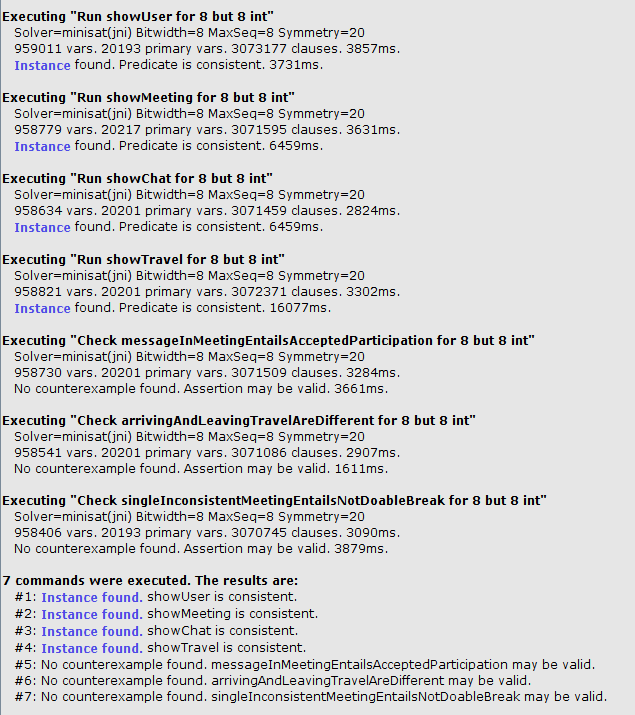
\includegraphics[width=\textwidth]{Images/AlloyResults.png}
	\caption{Execution of the Alloy model}
\end{figure}

\begin{figure}
	\vspace*{-0.5cm}
	\centering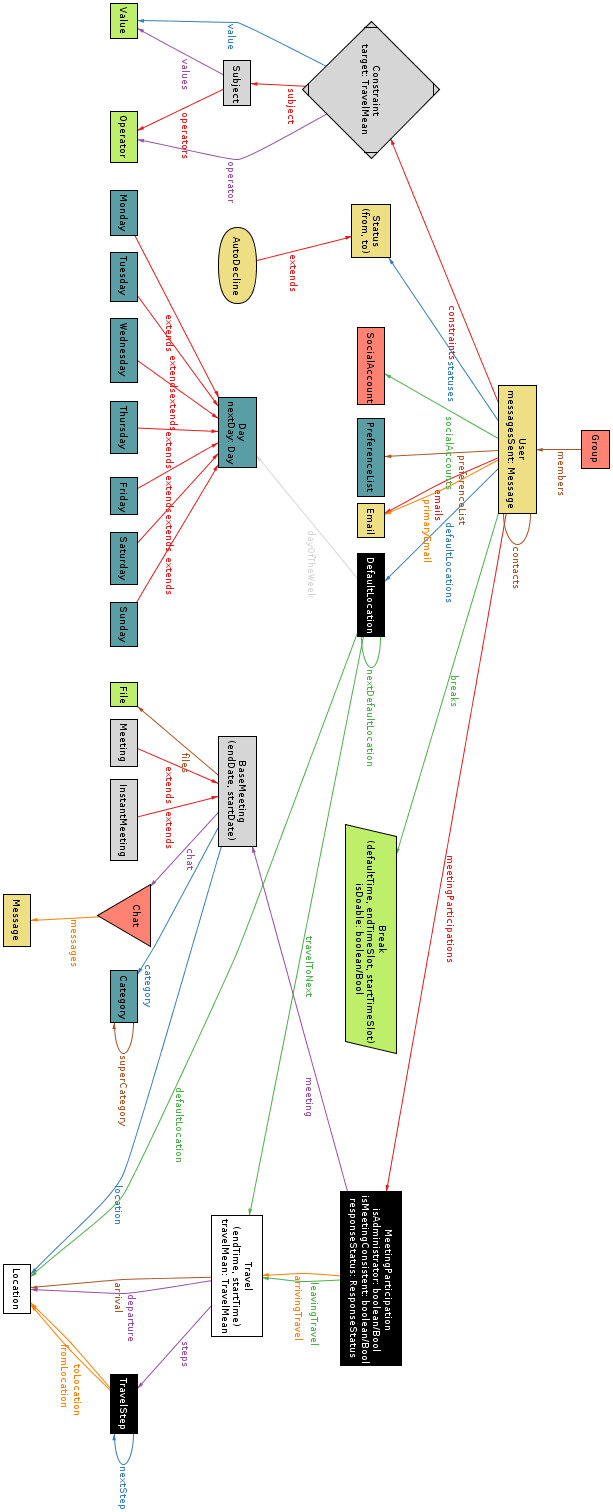
\includegraphics[height=\textheight]{Images/AlloyMetamodel.png}
	\caption{Execution of the Alloy model}
\end{figure}

\begin{figure}
	\vspace*{-0.5cm}
	\centering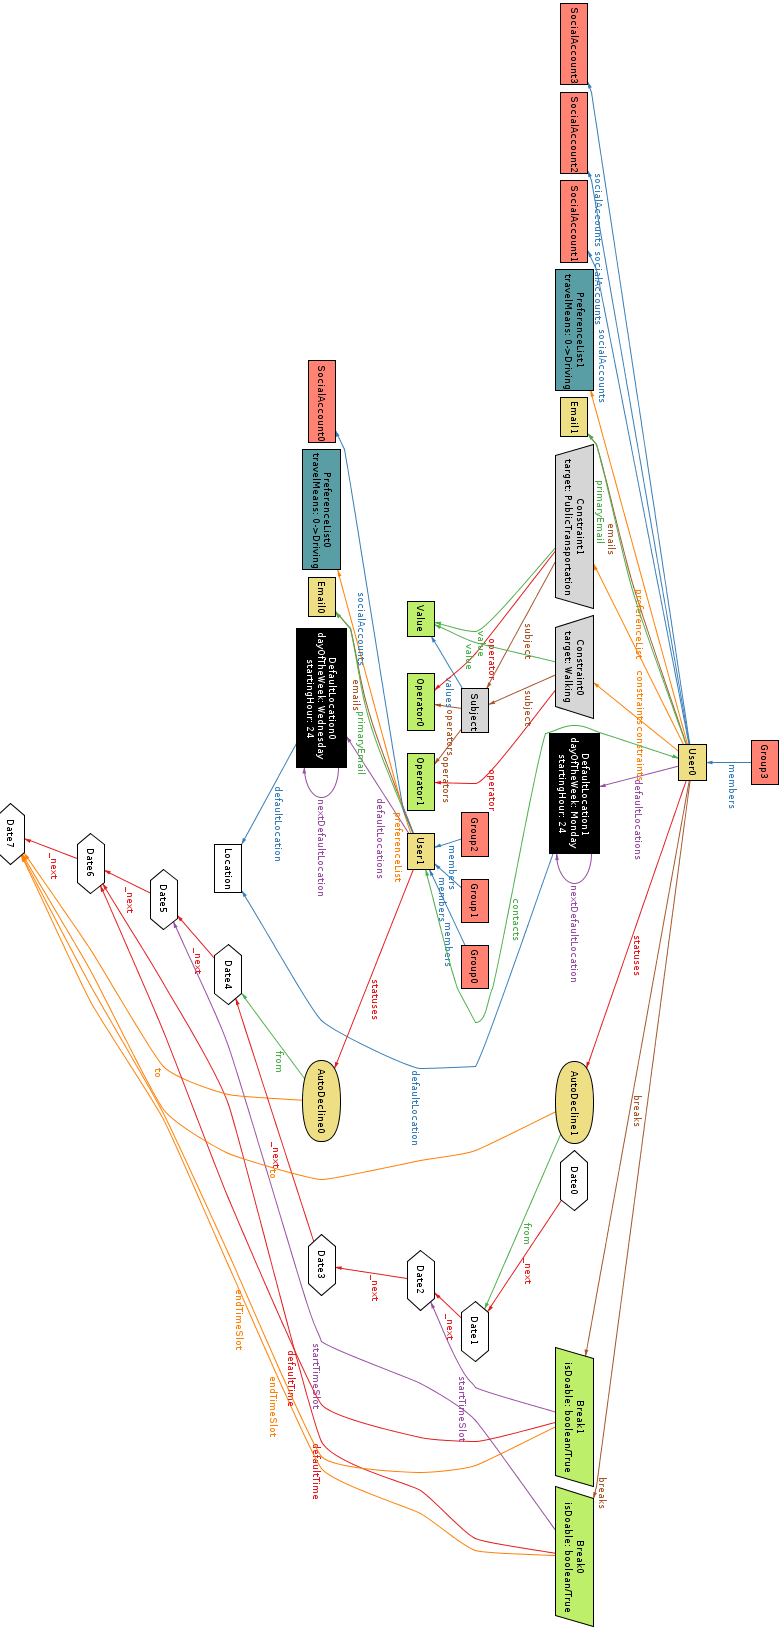
\includegraphics[height=\textheight]{Images/AlloyShowUser.png}
	\caption{Execution of the Alloy model}
\end{figure}

\begin{figure}
	\hspace*{-4cm}
	\centering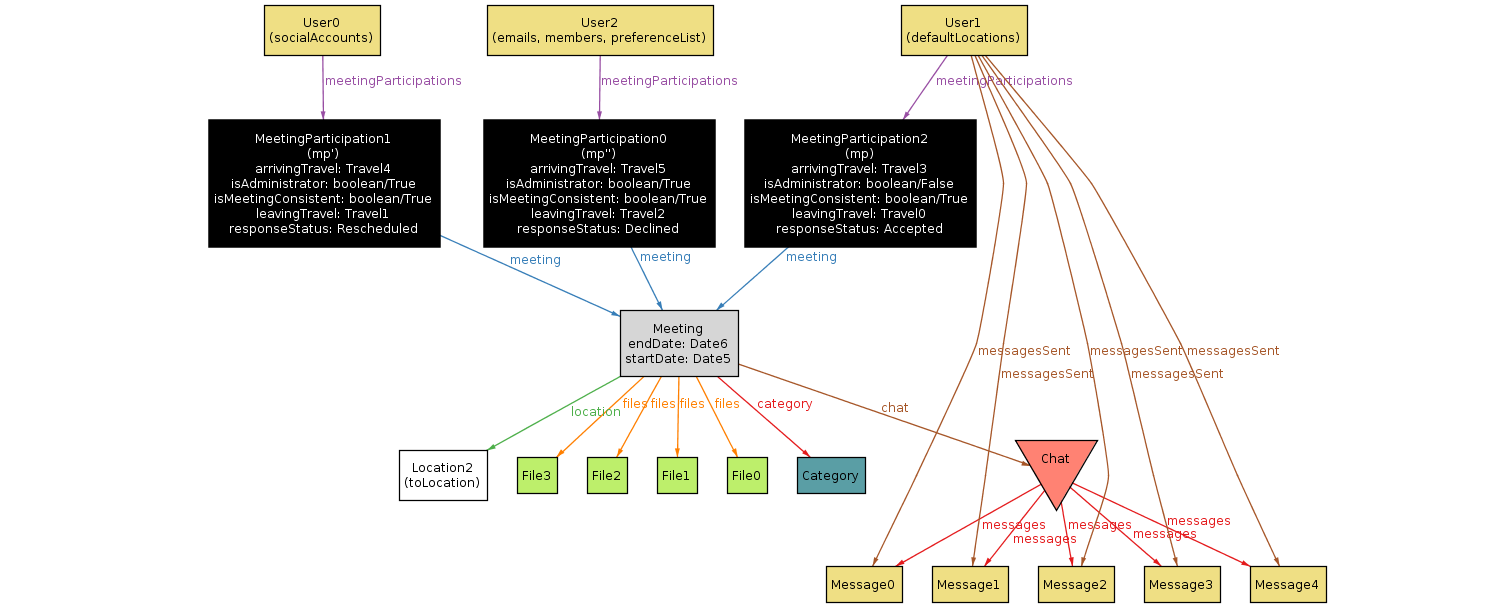
\includegraphics[scale=0.5]{Images/AlloyShowMeeting2.png}
	\caption{Execution of the Alloy model}
\end{figure}

\begin{figure}
	\hspace*{-2cm}
	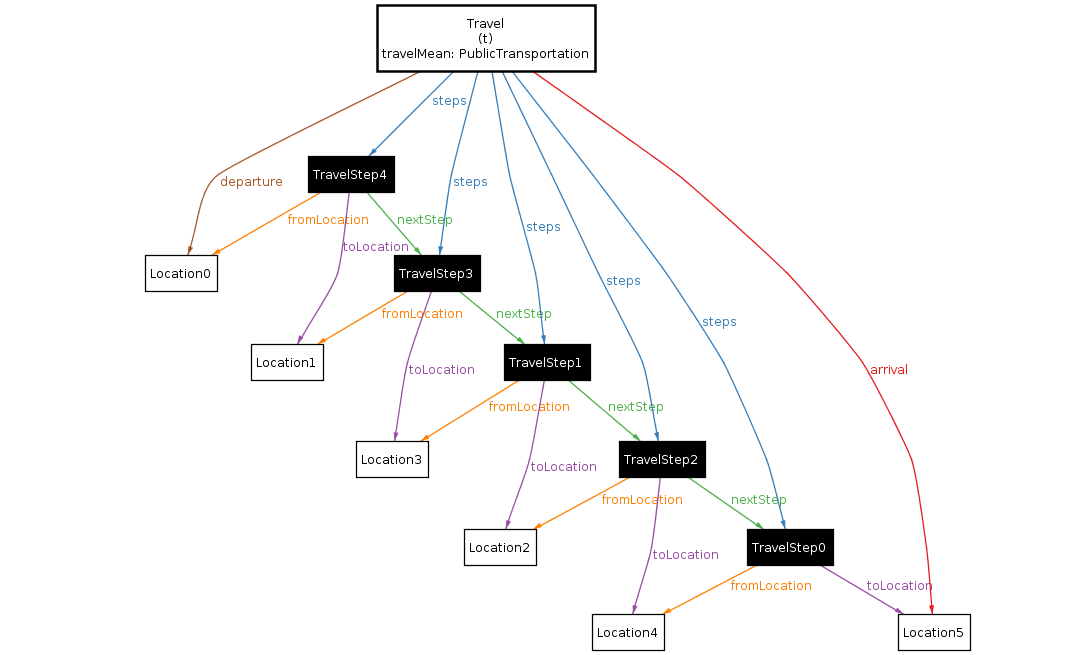
\includegraphics[scale=0.5]{Images/AlloyShowTravel2.png}
	\caption{Execution of the Alloy model}
\end{figure}